\documentclass[aps,prb,preprint,superscriptaddress,nofootinbib]{revtex4-2}

\usepackage{amsmath,amssymb,bm}
\usepackage{booktabs}
\usepackage{graphicx}

\newcommand{\T}{\mathbb T}
\newcommand{\ii}{\mathrm i}
\newcommand{\dd}{\mathrm d}
\newcommand{\sgn}{\operatorname{sgn}}

\begin{document}
\raggedbottom

\title{Exact indirect-gap boundary in a flux-one-third Harper--Hofstadter model with a period-three mass}

\author{Xiaojian Zeng}
\email{xiaojianzeng@foxmail.com}
\affiliation{PBC School of Finance, Tsinghua University, Beijing 100190, China}

\date{September 14, 2026}

\begin{abstract}
For a square-lattice Harper--Hofstadter Hamiltonian with flux $2\pi/3$,
anisotropic hoppings $t_x=1$ and $t_y=r$, and a magnetic-cell potential
$m(1,0,-1)$, a direct band touching does not in general coincide with the
fixed-filling metal--insulator boundary.  We determine both indirect gaps over
$1/2\leq r\leq2$ and all real $m$ by an exact computer-assisted calculation.
The gaps at one-third and two-thirds filling are equal.  Their common boundary
has an algebraic cusp at
$r_c=[(69-11\sqrt{33})/8]^{1/2}=0.852189\ldots$.  Below the cusp the only gap
zeros are the direct lines $m=\pm\sqrt3r$.  Above it, each direct line lies
strictly inside an indirect band-overlap window whose two edges are given by an
exact one-parameter algebraic representation.  A chemical-potential criterion
and Fej\'er--Riesz factorization reduce the global optimization over the
Brillouin torus to rational polynomial identities.  Sturm sequences exhaust
the physical and exceptional sectors, establishing that no further extrema
are missed.  The isolated-band Chern tuple is $(+1,-2,+1)$ for
$|m|<\sqrt3r$ and $(0,0,0)$ for $|m|>\sqrt3r$, even where an indirect overlap
makes the fixed-filling system metallic.
\end{abstract}

\maketitle

\section{Introduction}

At rational magnetic flux, the Harper equation becomes periodic and the
tight-binding spectrum splits into a finite set of magnetic subbands
\cite{Hofstadter1976}.  Their quantized Hall response is encoded by Chern
numbers \cite{TKNN1982}; the flux-one-third spectrum, its band topology, and
cold-atom realizations are reviewed in Ref.~\cite{Cooper2019}.  Experimental
superlattices can tune both the topology and separation of Hofstadter bands
\cite{Aidelsburger2015}.  These developments make it important to distinguish
two notions that coincide only in special models: isolation of adjacent bands
at every common momentum and a positive \emph{indirect} gap between their
global extrema.

This distinction matters at fixed filling.  An individual band can remain
isolated and carry a well-defined Chern number even when its maximum exceeds
the minimum of the next band at another momentum.  The system is then an
indirect metal rather than a band insulator.  Phase diagrams based solely on a
minimum same-momentum separation do not detect this overlap.  Related
commensurate Aubry--Andr\'e--Harper models, for example, have been classified
using direct-gap observables while varying diagonal and off-diagonal phason
modulations \cite{Ke2016}; that Hamiltonian and observable differ from the
static mass deformation considered here.

We solve the global problem for the three-band flux-one-third Hamiltonian with
the period-three onsite pattern $(m,0,-m)$.  The direct closures
$m=\pm\sqrt3r$ provide a useful baseline, but they are not the whole answer.
For sufficiently large anisotropy they sit inside finite indirect-overlap
windows.  The exact boundary of those windows has a cusp and two algebraic
branches.  The central technical point is to replace two independent global
band optimizations by the existence of a common chemical potential.  At a
boundary that condition becomes positivity of a degree-three trigonometric
polynomial, allowing a complete spectral-factor reduction and an exact Sturm
audit of every sector.

Section~\ref{sec:model} fixes the model and derives the momentum and spectral
symmetries.  Section~\ref{sec:result} states the complete boundary and its
extremizers.  Sections~\ref{sec:criterion}--\ref{sec:certificate} give the
factorization and completeness proof, and Sec.~\ref{sec:chern} gives the Chern
classification and physical limits.

\section{Model, global gaps, and exact reductions}
\label{sec:model}

We consider one noninteracting particle on an infinite square lattice with
lattice spacing one.  In Landau gauge the real-space Hamiltonian is
\begin{align}
\widehat H={}&-\sum_{x,y}\left(c^\dagger_{x+1,y}c_{x,y}
+r e^{2\pi\ii x/3}c^\dagger_{x,y+1}c_{x,y}+\mathrm{H.c.}\right)
\nonumber\\
&+\sum_{x,y}V_{x\bmod3}c^\dagger_{x,y}c_{x,y},
\qquad (V_{-1},V_0,V_{+1})=(m,0,-m).
\label{eq:realspace}
\end{align}
The energy unit is $t_x=1$, $r=t_y/t_x\in[1/2,2]$, and $m$ is real.  With
$\theta=k_y$ and magnetic-cell momentum $\kappa=3k_x$, both taken in
$[-\pi,\pi)$, the ordered sublattice basis $s=(-1,0,+1)$ gives
\begin{equation}
H_{r,m}(\theta,\kappa)=
\begin{pmatrix}
m-2r\cos(\theta-2\pi/3)&-1&-e^{-\ii\kappa}\\
-1&-2r\cos\theta&-1\\
-e^{\ii\kappa}&-1&-m-2r\cos(\theta+2\pi/3)
\end{pmatrix}.
\label{eq:bloch}
\end{equation}
This deformation is our model definition; it is not attributed to the
undeformed source Hamiltonian of Refs.~\cite{Hofstadter1976,Cooper2019}.

Let $E_1\leq E_2\leq E_3$ be the ordered eigenvalues.  At fillings $n/3$,
$n=1,2$, define
\begin{equation}
G_n(r,m)=\min_{\T^2}E_{n+1}-\max_{\T^2}E_n,
\qquad
d_n(r,m)=\min_{\T^2}(E_{n+1}-E_n).
\label{eq:gaps}
\end{equation}
Thus $G_n>0$ is the band-insulator condition, whereas $d_n>0$ only says that
the two bands are isolated at each momentum.

The matrix is traceless, and direct expansion gives the Chambers-type cubic
\begin{align}
P(E)&=\det(E-H)=E^3-AE-D,\label{eq:cubic}\\
A&=m^2+3r^2+3-2\sqrt3mr\sin\theta,\nonumber\\
D&=2m^2r\cos\theta-2\sqrt3mr^2\sin2\theta
-2r^3\cos3\theta-2\cos\kappa.\nonumber
\end{align}
For a simple ordered root at fixed $\theta$,
\begin{equation}
\frac{\partial E_j}{\partial D}=\frac{1}{3E_j^2-A}.
\label{eq:rootderivative}
\end{equation}
The denominator is positive for the two outer roots and negative for the
middle root.  Continuity extends the ordering through the already classified
double roots.  Because $D$ depends on $\kappa$ only through
$-2\cos\kappa$, all relevant $\kappa$ extrema lie at an endpoint:
\begin{align}
G_1&=\min_\theta E_2(\theta,\pi)-\max_\theta E_1(\theta,\pi),\nonumber\\
G_2&=\min_\theta E_3(\theta,0)-\max_\theta E_2(\theta,0).
\label{eq:kappareduction}
\end{align}
No finite momentum mesh enters this reduction.

The momentum-independent unitary
\begin{equation}
U=\begin{pmatrix}0&0&1\\0&-1&0\\1&0&0\end{pmatrix}
\end{equation}
obeys
\begin{equation}
H_{r,m}(\pi-\theta,\pi-\kappa)
=-U H_{r,m}(\theta,\kappa)U^\dagger.
\label{eq:spectralreflection}
\end{equation}
It follows that
$E_j(\pi-\theta,\pi-\kappa)=-E_{4-j}(\theta,\kappa)$ and hence
\begin{equation}
\boxed{G_1(r,m)=G_2(r,m)\equiv G(r,m).}
\label{eq:gapequality}
\end{equation}
The characteristic polynomial is also invariant under
$(m,\theta)\mapsto(-m,-\theta)$, so $G$ is even in $m$.

For reference, the only direct degeneracies are
\begin{equation}
(m,\theta)=(+\sqrt3r,+\pi/2),\quad
(-\sqrt3r,-\pi/2),
\label{eq:directmass}
\end{equation}
with $\kappa=0$ for the upper gap and $\kappa=\pi$ for the lower gap.
Indeed, subtracting a double eigenvalue from a $3\times3$ Hermitian matrix
makes it rank one.  The three off-diagonal magnitudes in Eq.~\eqref{eq:bloch}
are all unity, so rank-one factorization forces the three shifted diagonal
entries to agree; tracelessness then forces the original diagonals to vanish.
Solving those equations gives Eq.~\eqref{eq:directmass}.  The remaining
zero-diagonal ring has polynomial $E^3-3E+2\cos\kappa$, whose discriminant
vanishes only at $\kappa=0,\pi$.

\section{Complete indirect-gap boundary}
\label{sec:result}

We first give a square-root-free parametrization of the positive-mass
indirect boundary.  For $X\in(3/4,1)$ define
\begin{align}
A_X&=8X^2-4X-1,&
B_X&=40X^3-36X^2+6X-1,\nonumber\\
V(X)&=\frac{3(2X-1)^2A_X}{4B_X},
\label{eq:V}\end{align}
and
\begin{align}
e_0(X)&=-\frac{(2X-1)(16X^3-60X^2+36X-1)}{2B_X},\label{eq:e0}\\
k_0(X)&=-\frac{(X-1)(2X-1)(2X+1)^2(4X-3)(4X-1)^2}
{6A_XB_X^2}
\nonumber\\[-2mm]
&\hspace{20mm}\times(28X^2-20X+1)^2,\label{eq:k0}\\
a(X)&=\frac{k_0(X)V(X)}{X}.
\end{align}
Let $Y_+(X)$ be the unique positive root satisfying $e_0Y\geq1$ of
\begin{equation}
a(X)Y^3-3e_0(X)Y+2=0.
\label{eq:Ycubic}
\end{equation}
Away from the cusp the inequality is strict.  Set
\begin{align}
r(X)&=Y_+(X)\sqrt{\frac{V(X)}{X}},\label{eq:rparam}\\
u(X)&=\frac{4\sqrt{V(X)(1-X)}(4X-1)}{3(2X-1)},\nonumber\\
m(X)&=\sqrt3\,u(X)r(X),\qquad E(X)=e_0(X)Y_+(X).
\label{eq:mparam}
\end{align}

The two branches meet at
\begin{equation}
X_c=\frac{7+\sqrt{33}}{16},\qquad
r_c=\sqrt{\frac{69-11\sqrt{33}}8}
=0.852189157998510\ldots,
\label{eq:cusp}
\end{equation}
where $u=1$, $E=1$, and $m=\sqrt3r_c$.  The function $r(X)$ decreases
strictly from infinity to $r_c$ on $(3/4,X_c)$ and increases strictly from
$r_c$ to infinity on $(X_c,1)$.  Therefore, for every $r>r_c$, there are
exactly two inverse values
\begin{equation}
X_<(r)\in(3/4,X_c),\qquad X_>(r)\in(X_c,1).
\end{equation}
Define
\begin{equation}
m_+(r)=m[X_<(r)],\qquad m_-(r)=m[X_>(r)].
\label{eq:mpm}
\end{equation}
They obey $0<m_-<\sqrt3r<m_+$.

The main result is the following complete sign classification:
\begin{equation}
\begin{array}{ll}
\frac12\leq r\leq r_c:&
G>0\ \text{for}\ m\neq\pm\sqrt3r,
\quad G=0\ \text{at}\ m=\pm\sqrt3r;\\[1mm]
r_c<r\leq2:&
G<0\ \Longleftrightarrow\ m_-(r)<|m|<m_+(r),\\
&G=0\ \Longleftrightarrow\ |m|=m_-(r)\ \text{or}\ m_+(r),
\end{array}
\label{eq:classification}
\end{equation}
with $G>0$ otherwise.  Thus the relative boundary of the insulating set
consists of the two direct segments $m=\pm\sqrt3r$ for
$1/2\leq r\leq r_c$, joined at the cusps to the four mass-reflected
indirect branches $m=\pm m_\pm(r)$ for $r_c\leq r\leq2$.  For $r>r_c$ the
direct line is a Chern-changing band touching \emph{inside} the metallic
window and is not a boundary of the fixed-filling insulating set.

Figure~\ref{fig:phase} shows this distinction.  Selected evaluations of the
exact parametrization are listed in Table~\ref{tab:boundary}; the displayed
digits are not used in the proof.

\begin{figure}[t]
\centering
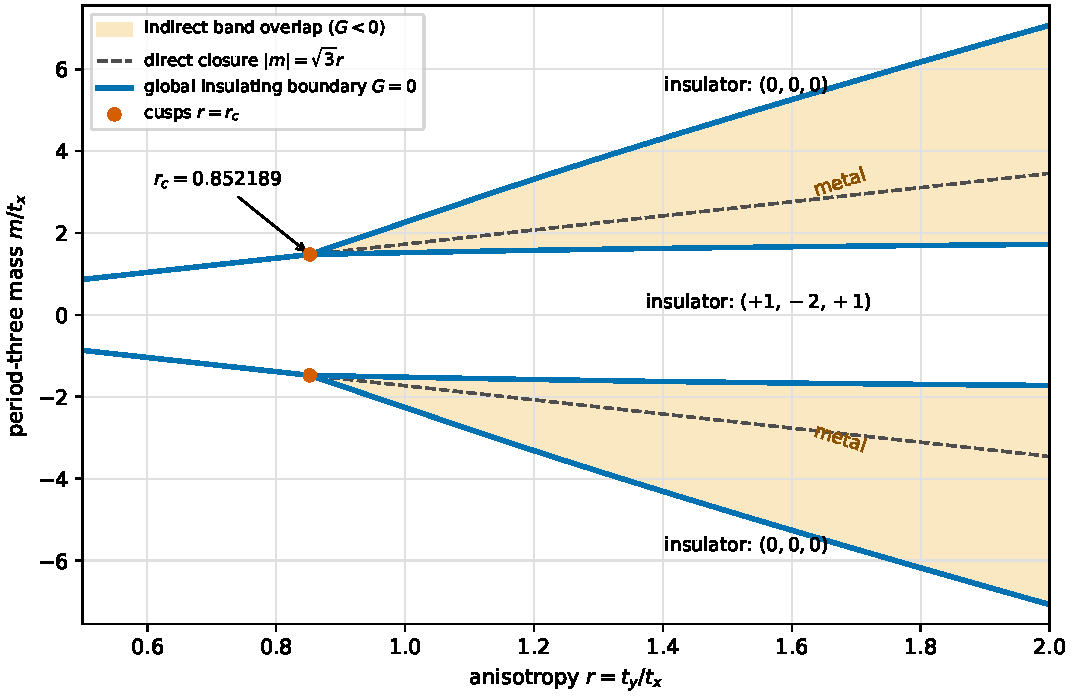
\includegraphics[width=0.95\linewidth]{../figures/phase_diagram.pdf}
\caption{Global fixed-filling diagram for either $1/3$ or $2/3$ filling.
Blue curves are the exact $G=0$ boundary, orange regions have indirect
overlap $G<0$, and unshaded regions have $G>0$.  The dashed direct closures
continue through the metallic windows and change the isolated-band Chern
tuple there.  The vector plot is a deterministic evaluation of
Eqs.~\eqref{eq:V}--\eqref{eq:mpm}; AI assisted in drafting the plotting code,
whose coordinates were checked against the exact formulas and Table~\ref{tab:boundary}.}
\label{fig:phase}
\end{figure}

\begin{table}[b]
\caption{Positive-mass indirect boundaries.  Values are numerical
evaluations of the exact parametrization.}
\label{tab:boundary}
\begin{ruledtabular}
\begin{tabular}{c@{\qquad}cc}
$r$ & $m_-(r)$ & $m_+(r)$\\
\colrule
0.90 & 1.491168750337 & 1.732042744620\\
1.00 & 1.522145273973 & 2.269195105327\\
1.25 & 1.591352307724 & 3.569738391484\\
1.50 & 1.646066824501 & 4.789938828072\\
2.00 & 1.721949718751 & 7.074701110742\\
\end{tabular}
\end{ruledtabular}
\end{table}

The global extremizers are also fixed by the parametrization.  For positive
$m$, set
\begin{equation}
\phi=-\arccos\sqrt X,\qquad
\delta=\arccos[-\sqrt{V(X)}],\qquad
\theta_c=\phi+\delta,\quad\theta_v=\phi-\delta.
\label{eq:angles}
\end{equation}
At filling $2/3$, $(\theta_c,0)$ is the $E_3$ minimum and
$(\theta_v,0)$ is the $E_2$ maximum.  At filling $1/3$, the corresponding
conduction and valence momenta are $(\pi-\theta_v,\pi)$ and
$(\pi-\theta_c,\pi)$.  Negative mass negates every $\theta$ coordinate.
On a direct segment the contact is at $\theta=\sgn(m)\pi/2$, with
$\kappa=0$ for $2/3$ filling and $\kappa=\pi$ for $1/3$ filling.  At the
cusp Eq.~\eqref{eq:angles} includes the direct contact and a distinct-momentum
global extremum, so the two kinds of closure meet without being conflated.

\section{Chemical-potential criterion}
\label{sec:criterion}

It remains to prove that Eqs.~\eqref{eq:classification} and
\eqref{eq:angles} are exhaustive.  Put $q=m/\sqrt3$ and initially take
$m\geq0$.  At $\kappa=0$, Eq.~\eqref{eq:cubic} becomes
\begin{align}
f_{E,r,q}(\theta)={}&E^3-3E(1+r^2+q^2)+2
+6Eqr\sin\theta-6q^2r\cos\theta\nonumber\\
&+6qr^2\sin2\theta+2r^3\cos3\theta.
\label{eq:f}
\end{align}
For general $K=\cos\kappa$,
$P_K(E,\theta)=f_{E,r,q}(\theta)+2(K-1)\leq f_{E,r,q}(\theta)$.

Every Bloch matrix has $E_3\geq1$ and $E_1\leq-1$.  To see this, note that
$\operatorname{tr}H^2=2A\geq6$.  For a traceless ordered triple whose largest
entry is $M$, direct optimization of the other two entries gives
$\sum_jE_j^2\leq6M^2$; applying the same statement to $-H$ gives both bounds.
For $E\geq1$, the condition $P_K(E,\theta)\leq0$ is therefore equivalent to
$E_2(\theta,\kappa)\leq E\leq E_3(\theta,\kappa)$.  Combining this fact with
Eq.~\eqref{eq:kappareduction} yields the exact intersection criterion
\begin{equation}
G_2\geq0\quad\Longleftrightarrow\quad
\exists E\geq1\ \text{such that}\ f_{E,r,q}(\theta)\leq0
\ \text{for all}\ \theta.
\label{eq:criterion}
\end{equation}
Strict inequalities characterize $G_2>0$.  At a genuinely indirect zero,
$h(\theta)=-f(\theta)$ is a nonnegative degree-three trigonometric polynomial
with two distinct zeros, the conduction and valence momenta.  This turns the
global band comparison into an exact positivity problem.

\section{Spectral factorization and algebraic reduction}
\label{sec:factorization}

Let $z=e^{\ii\theta}$ and let $z_c,z_v$ be the two unit-circle zeros of $h$.
Fej\'er--Riesz factorization gives
\begin{equation}
h(\theta)=\left|\alpha(z-z_c)(z-z_v)(z-\zeta)\right|^2.
\label{eq:FR}
\end{equation}
The third Fourier coefficient is $-r^3$.  Replacing the spectral factor by
its reciprocal if necessary permits
\begin{equation}
\zeta=\frac{\rho}{z_cz_v},\qquad \rho\geq1,\qquad
|\alpha|^2=\frac{r^3}{\rho},\qquad t=\rho+\rho^{-1}\geq2.
\end{equation}
Write
\begin{equation}
\phi=\frac{\theta_c+\theta_v}{2},\quad
\delta=\frac{\theta_c-\theta_v}{2},\quad v=\cos\delta,
\quad u=\frac qr,\quad e=\frac Er.
\end{equation}
Direct autocorrelation of Eq.~\eqref{eq:FR} and matching the second and first
Fourier coefficients of Eq.~\eqref{eq:f} gives
\begin{align}
4v\cos\phi+t\cos2\phi&=0,&
4v\sin\phi-t\sin2\phi&=3u,\label{eq:match1}\\
\operatorname{Re}W&=-3u^2,&
\operatorname{Im}W&=-3ue,\label{eq:match2}
\end{align}
where
\begin{equation}
W=(2+4v^2)e^{2\ii\phi}+4tv e^{-\ii\phi}+e^{-4\ii\phi}.
\end{equation}
The constant autocorrelation is
\begin{equation}
H=2(1+2v^2)t+8v\cos3\phi,
\end{equation}
and its matching equation is
\begin{equation}
[H+e^3-3e(1+u^2)]r^3-3er+2=0.
\label{eq:constantmatch}
\end{equation}
No energy equation or stationarity condition has been squared in this
derivation.

The representation redundancy $(\phi,v)\mapsto(\phi+\pi,-v)$ allows
$\cos\phi>0$.  In the positive-mass two-angle sector the equations then fix
$\sin\phi<0$ and $v<0$.  Put $X=\cos^2\phi$ and $V=v^2$.  Solving the two
linear equations \eqref{eq:match1}, reducing Eq.~\eqref{eq:match2} modulo
$\cos^2\phi+\sin^2\phi=1$, and eliminating even powers produces a single
primitive relation,
\begin{align}
0={}&-160VX^3+144VX^2-24VX+4V\nonumber\\
&+96X^4-144X^3+60X^2-3.
\label{eq:primitive}
\end{align}
It is linear in $V$ and solves uniquely to Eq.~\eqref{eq:V}.  The remaining
matches give Eqs.~\eqref{eq:e0}--\eqref{eq:Ycubic}.  Thus the displayed
one-parameter curve is not a fit to a momentum scan; it is the generic real
solution of the full Fourier matching ideal.

At a zero of $P$, the sign of $P_E=3E^2-A$ distinguishes the ordered band.
On both open branches the two factor zeros obey
\begin{equation}
P_E(\theta_c)>0>P_E(\theta_v).
\label{eq:PEsigns}
\end{equation}
Together with $h\geq0$, this proves that they are respectively the global
$E_3$ minimum and $E_2$ maximum, rather than two extrema of one band.

\section{Exact completeness certificate}
\label{sec:certificate}

We summarize the exact sector and monotonicity certificate; Appendix
\ref{app:certificate} gives its decisive polynomials.  The first matching
equations imply
\begin{equation}
t^2=\frac{16XV}{(2X-1)^2},\qquad
t^2-4=\frac{4(1-X)(4X-1)^2}{B_X}.
\label{eq:tsector}
\end{equation}
The requirements $t\geq2$ and $0<V<1$ first reduce the generic sector to the
part above the sole relevant zero of $B_X$.  In the remaining possible
interval below $X=3/4$, $e_0>0$ while the cubic coefficient corresponding to
$k_0$ is nonpositive.  The constant-match cubic is strictly decreasing for
positive $r$, and at $E=1$ it is already negative.  Its unique positive root
therefore has $E<1$ and is excluded by Eq.~\eqref{eq:criterion}.  Every
generic physical contact consequently satisfies
\begin{equation}
\frac34<X<1.
\label{eq:Xsector}
\end{equation}

On this interval Eq.~\eqref{eq:Ycubic} has one negative and two positive
roots, with exactly one root satisfying $E=e_0Y\geq1$ except for their
coalescence at the cusp.  The exact sign identity
\begin{align}
e_0^3-a={}&\frac{3(2X-1)^3A_X(16X^2-14X+1)^2}{8XB_X^3}\nonumber\\
&\times(32X^4-8X^3-36X^2+22X-1)
\end{align}
locates that root without a numerical branch choice.  Rational Sturm
sequences show that all displayed factors have the required fixed signs.

For monotonicity, impose Eq.~\eqref{eq:Ycubic} and differentiate
$r=Y\sqrt{V/X}$.  After denominator and endpoint factors are removed, the
stationarity resultant contains only
\begin{equation}
(16X^2-14X+1)^2S_{12}(X).
\label{eq:stationaryfactors}
\end{equation}
The first factor has the physical root $X_c$ in Eq.~\eqref{eq:cusp}.  An
exact Sturm count finds one root of $S_{12}$ in $(3/4,1)$, isolated in
$(0.769,0.770)$; substituting its exact rational expression for $Y$ proves
$Y<0$.  It belongs to the negative cubic root and cannot make the physical
branch stationary.  Endpoint limits give $r(X)\to\infty$ on both sides of
the interval, proving the stated two-branch monotonicity.

No division sector is discarded silently.  If $\cos\phi=0$, the first
matching equation would give $t=0$; $X=1/2$ or $v=0$ gives
$t=\sqrt3<2$; $\sin\phi=0$, $u=0$, or $t=2$ reduces to the massless
sector.  At $m=0$ the choice $E=\sqrt{1+r^2}$ lies strictly inside the gap
because
\begin{equation}
(1+r^2)^3-(1+r^3)^2=r^2(3r^2-2r+3)>0.
\end{equation}
A coincident pair of contact angles, a single unit-circle zero, or a unit
third factor reduces to either this massless endpoint or the direct
degeneracies already classified in Eq.~\eqref{eq:directmass}.  Negative mass
is covered by exact reflection.

Exact algebraic-root isolation at one rational point on each open branch
proves Eq.~\eqref{eq:PEsigns}.  Its sign cannot change before the cusp because
$P_E=0$ would be an additional direct degeneracy, already excluded.  Finally,
the exhaustive zero classification and continuity determine the signs in
Eq.~\eqref{eq:classification}: the undeformed and large-mass components have
positive gap, while direct substitution on $m=\sqrt3r$ gives a negative
sample for $r>r_c$.  This closes the global argument, including parameter
edges and exceptional sectors.

All decisive polynomial operations use exact integer or rational arithmetic,
with the explicit quadratic field $\mathbb Q(\sqrt{33})$ at the cusp.  The
machine-readable certificate reconstructs the Laurent coefficients directly
from Eq.~\eqref{eq:bloch}, derives Eq.~\eqref{eq:primitive} without importing
$V(X)$, factors the resultants, performs the Sturm counts, and asserts every
exceptional-sector identity.  Floating-point diagonalization is used only as
an independent replay and for Fig.~\ref{fig:phase}; it is not the source of
exhaustiveness.

OpenAI Codex (a GPT-5-based agent, September 2026 service version) assisted
with problem formulation, literature synthesis, symbolic derivations, and
generation and debugging of the verification code.  It was directed by the
fixed Hamiltonian and explicit exact-arithmetic assertions.  Outputs were
cross-checked using two independently constructed Bloch representations,
coefficient-by-coefficient Laurent reconstruction, rational Sturm sequences,
and a separately implemented numerical replay.  These computational checks
are not a substitute for human peer review; final human scientific review is
required before submission.

\section{Chern labels and physical scope}
\label{sec:chern}

Equation~\eqref{eq:directmass} proves that the three individual bands can
change Chern number only on $m=\pm\sqrt3r$.  The central parameter region is
connected to $r=1,m=0$, whose positive-flux, energy-ordered tuple is
$(+1,-2,+1)$ \cite{Cooper2019}.  It is also reproduced by converged
link-variable and independent Kubo-curvature calculations.  Each outer region
can be deformed to large $|m|$ without crossing a direct closure.  For
$|m|>4(r+1)$, scale all hoppings by $\lambda\in[0,1]$.  Gershgorin intervals
of radius $2\lambda(r+1)$ around the onsite energies $-m,0,+m$ remain
disjoint.  At $\lambda=0$ the projectors are constant atomic-sublattice
projectors, so every Chern number vanishes.  Hence
\begin{equation}
(C_1,C_2,C_3)=
\begin{cases}
(+1,-2,+1),&|m|<\sqrt3r,\\
(0,0,0),&|m|>\sqrt3r.
\end{cases}
\label{eq:chern}
\end{equation}
Complex conjugation or orientation reversal changes the nonzero tuple to
$(-1,+2,-1)$ and leaves the zero tuple unchanged.

The dashed portions of Fig.~\ref{fig:phase} illustrate why Chern labels and
fixed-filling insulation must be reported separately.  On either side of a
direct closure inside an orange window, the bands are again individually
isolated and Eq.~\eqref{eq:chern} applies, but $G<0$ and neither filling is a
band insulator.

The result is restricted to the infinite, clean, noninteracting
single-particle Hamiltonian in Eq.~\eqref{eq:bloch}.  It does not include
interactions, disorder, trapping, edges, finite-size corrections, or an
experimental error budget, and it is not a claim about a many-body
thermodynamic transition.  The exact certificate is computer assisted rather
than formalized in a proof assistant.  A bounded comparison with period-three
superlattice, generalized Harper, and commensurate Aubry--Andr\'e--Harper
literature found no identical static-mass global boundary, but this
non-detection is not an exhaustive priority claim and warrants broader human
literature review.

\section{Conclusion}

The global insulating boundary of this flux-one-third mass-deformed
Harper--Hofstadter model is qualitatively different from its direct-gap phase
diagram.  An exact chemical-potential factorization reveals an algebraic cusp
at $r_c$ and, above it, two mass edges surrounding each direct topological
closure.  Exact sector elimination and Sturm counts prove that these are all
the edges over the full Brillouin torus and parameter domain.  The resulting
diagram cleanly separates the Chern topology of isolated bands from the
existence of a fixed-filling band insulator.

\begin{acknowledgments}
OpenAI Codex (a GPT-5-based agent, September 2026 service version) also
assisted with literature organization, manuscript drafting, and deterministic
data-visualization code.  The scientific uses, direction, and computational
cross-checks are described in Sec.~\ref{sec:certificate}.  The human author
must review and refine all content, verify the disclosure against the current
APS policy and applicable service terms, and accept responsibility before any
submission.  No external peer review or editorial assessment has occurred.
\end{acknowledgments}

\section*{Data Availability}

The complete LaTeX source, exact-arithmetic verification scripts, generated
boundary data, figure-generation code, software versions, and regeneration
instructions are included in the accompanying reproducibility archive.  The
CSV data are a sampled visualization of the exact equations, not the
definition of the boundary.

\appendix

\section{Decisive stationary polynomial}
\label{app:certificate}

For completeness, the degree-12 factor in
Eq.~\eqref{eq:stationaryfactors} is
\begin{align}
S_{12}(X)={}&602112X^{12}-1505280X^{11}+1069824X^{10}
+184576X^9\nonumber\\
&-524928X^8+195264X^7-23328X^6+8736X^5
-3528X^4\nonumber\\
&+228X^3-45X^2+15X-1.
\end{align}
At its sole root in $(0.769,0.770)$, the simultaneous stationary solution is
\begin{equation}
Y=-\frac{2B_XP_5(X)}{X(2X-1)P_7(X)},
\end{equation}
where
\begin{align}
P_5={}&224X^5-296X^4+76X^3+10X^2+5X-1,\\
P_7={}&3584X^7-23296X^6+38688X^5-24304X^4\nonumber\\
&+5024X^3-96X^2+182X-25.
\end{align}
Exact root counts show that $B_X,P_5,P_7$ have no zero in the isolating
interval and have the signs that make $Y<0$.  The full numerator resultant,
up to a nonzero rational factor, is
\begin{equation}
(4X-1)^2X^3(2X-1)^3A_X(16X^2-14X+1)^2
{}\times(28X^2-20X+1)^2B_X^9S_{12}(X).
\end{equation}
The factors outside $(3/4,1)$ or already known to be nonzero on that interval
are retained here to make the division structure explicit.

\section{Undeformed benchmark}

At $r=1,m=0$, Eq.~\eqref{eq:cubic} reduces to
\begin{equation}
P(E)=E^3-6E+2[\cos(3\theta)+\cos\kappa].
\end{equation}
Because the bracket fills $[-2,2]$, the three exact band ranges are
\begin{equation}
E_1\in[-1-\sqrt3,-2],\quad
E_2\in[1-\sqrt3,\sqrt3-1],\quad
E_3\in[2,1+\sqrt3].
\end{equation}
Both direct gaps are therefore $3-\sqrt3$.  This reproduces a source-anchored
limit independently of the indirect-boundary calculation.

\bibliography{references}

\end{document}
